%\paragraph{Transport Layer Security (TLS).}
TLS~\cite{rfc5246} is one of the main protocols
responsible for transport security on the modern Internet.
%Properly
%used, TLS prevents eavesdropping, tampering, or message forgery in
%communications between client and server applications such as web and
%email traffic.
TLS and its precursor SSLv3 have been the target of a large number of cryptographic attacks in
the research community, both on popular implementations and the
protocol itself~\cite{2013:01:briefChronologyOfSSLTLSAttacks}.
Prominent recent examples include attacks on outdated or deliberately
weakened encryption in RC4~\cite{RC4biases}, RSA~\cite{SMACKTLS}, and
Diffie-Hellman~\cite{LogJam}, different side channels including
Lucky13~\cite{Lucky13}, BEAST~\cite{BEAST}, and POODLE~\cite{POODLE},
and several attacks on invalid TLS protocol
flows~\cite{SMACKTLS,ProtocolStateFuzzing15,TripleHandshake}.

Comparatively little attention has been paid to the \ssltwo protocol,
likely because the known attacks are so devastating and the protocol
has long been considered obsolete.  Wagner and Schneier wrote in 1996 that
their attacks on \ssltwo ``will be irrelevant in the long term
when servers stop accepting SSL 2.0 connections''~\cite{WagnerSchneier:SSLAnalysis:96}.
Most modern TLS clients do not support \ssltwo at all.
However, in Internet-wide scans we found that out of 36~million
HTTPS servers, 6~million (17\%) support \ssltwo.

%However, a surprisingly large number
%of servers, including 16\% of all HTTPS servers, 5\% of those HTTPS servers
%running browser-trusted certificates, and 36\% of SMTP servers
% still support \ssltwo.  

%\paragraph{Bleichenbacher's attack.}
Bleichenbacher's padding oracle attack~\cite{Bleichenbacher} is an
adaptive chosen ciphertext attack against RSA \PKCS, the RSA padding
standard used in TLS\@.  This attack enables decryption of RSA-encrypted
ciphertexts if a server distinguishes between correctly and
incorrectly padded RSA plaintexts, and was termed the
``million-message attack'' upon its introduction in 1998 after the
number of RSA decryption queries needed to deduce a plaintext.  All
widely-used modern SSL/TLS server implementations include
countermeasures against Bleichenbacher attacks.

\if0
\paragraph{Our results.}
In this paper, we construct an efficient Bleichenbacher attack~\cite{Bleichenbacher}
against \ssltwo that needs only a few thousand server queries to
decrypt an RSA ciphertext.
Our attack works against implementations that
implement the recommended countermeasures against Bleichenbacher attacks.  Next, we go on to show how
our \ssltwo attack can be used to decrypt passively collected TLS
ciphertexts from clients who do not even speak \ssltwo.  Due to
widespread reuse of RSA keys across servers, protocols, and protocol
versions, an attacker can use our attack to compromise completely
up-to-date clients and servers.
\fi

\paragraph{A Bleichenbacher attack on \ssltwo.}
Our first result shows that the \ssltwo protocol is fatally
vulnerable to a form of Bleichenbacher attack
%Bleichenbacher adaptive chosen ciphertext
%attack~\cite{Bleichenbacher} 
that enables decryption of RSA
ciphertexts.  We develop a novel application of the
attack that allows us to use a server that supports \ssltwo as an
efficient padding oracle.  This attack is a protocol-level flaw in \ssltwo that
results in a feasible attack for 40-bit export cipher strengths,
and in fact abuses the universally implemented countermeasures against
Bleichenbacher attacks to obtain a decryption oracle.

We also discovered multiple implementation flaws in
commonly deployed OpenSSL versions that allow an extremely efficient
and much more dangerous instantiation of this attack.

\if0
Our attack exploits two
properties of the \ssltwo protocol:
\begin{enumerate}
	\item In \ssltwo the
	client-generated \texttt{secret\_key\_data} may vary in
	length, and can be as short as five bytes for export cipher
	suites.  The client encrypts this value to the server's public
	RSA key and sends it to the server in a client key exchange
	message.  The client and server then both derive symmetric
	encryption and authentication keys from this value.  In SSLv3
	and later versions of TLS the client-generated key material
	(called the \pms) is always 48 bytes in length, even for
	40-bit export cipher suites.

        \item In \ssltwo the server
	sends its \texttt{ServerVerify} authentication message
	immediately after receipt of the client key exchange.  In
	contrast, in SSLv3 and later versions of TLS the server does
	not send its server \texttt{Finished} authentication message
	until after it has received and validated the
	client \texttt{Finished} message, proving that the client
	knows the negotiated \pms.
\end{enumerate}

Our attack also relies on the universally implemented countermeasure
against Bleichenbacher attacks.  Namely, an SSL/TLS server
implementation that receives an RSA key exchange message with invalid
padding will carry out the
rest of the TLS handshake using a randomly generated premaster secret.

To obtain a Bleichenbacher padding oracle, an attacker initiates
two \ssltwo connections to the victim server, negotiates a weak
symmetric cipher (e.g.~40-bit export RC2), and sends identical RSA
ciphertexts for both the client key exchanges.  He receives
two \texttt{ServerVerify} messages in response, each encrypted using
the derived session key.  He then performs an offline brute force
search on the \texttt{secret\_key\_data}. One of
the \texttt{secret\_key\_data} values will correctly decrypt
the \texttt{ServerVerify} message for the first connection. If the
same value also correctly decrypts the \texttt{ServerVerify} message
for the second connection, the attacker can deduce with high
probability that the RSA ciphertexts contained valid padding, as the
server was able to derive the same encrypted value from both.
Otherwise, the attacker can deduce that the RSA padding was invalid
and the server employed the standard anti-Bleichenbacher
countermeasure of generating a random \texttt{secret\_key\_data} for
each connection.

The attack as we have presented it allows us to extract a session key
from an \ssltwo handshake using a weak symmetric cipher.  This does
not pose much additional practical security risk to \ssltwo, as the
protocol is known to be vulnerable to devastating man-in-the-middle
attacks, and a passive attacker could have simply used brute force to
compute the weak symmetric key in the first place.  However, this
vulnerability can be strengthened into an attack on modern TLS
clients.

%This widespread \ssltwo support has so far not been seen as a critical security risk, as the majority of SSL/TLS clients will simply refuse to initiate \ssltwo connections \cite{holz_ndss_2016}; the perception that \ssltwo support is not a critical security concern is apparently one of the reasons for the widespread support of this officially prohibited~\cite{ProhibitingSSLv2} protocol. 

%\todo{I'm not sure what exactly we're trying to say here... (Nimrod)}
%Another evidence of the \ssltwo relevance provide recent vulnerability fixes in the OpenSSL \ssltwo source code files. For example, a countermeasure against a timing-based Bleichenbacher attack was provided in \todo{add year or fix, if relevant}.  This also means that \ssltwo implementations are not vulnerable to a timing attack.

\begin{figure}[t]
	%\centering 
	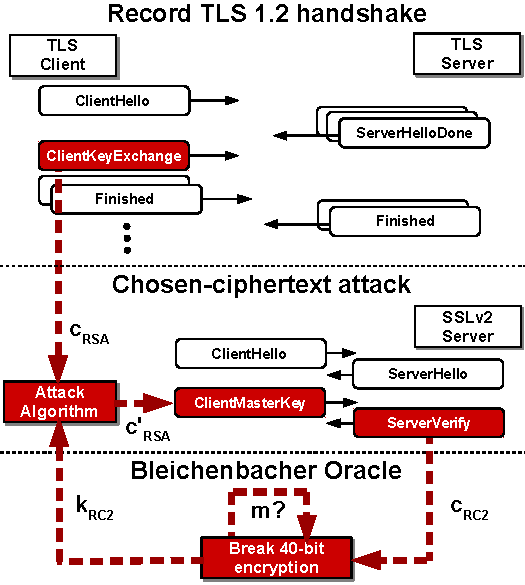
\includegraphics[width=0.5\textwidth]{img/ssl-tls} 
	\caption{\textbf{Our \ssltwo-based Bleichenbacher attack on TLS.} An attacker passively collects RSA ciphertexts from a TLS 1.2 handshake, and then performs oracle queries against a server that supports \ssltwo with the same public key to decrypt the TLS ciphertext.}
	\label{fig:ssl-tls}
\end{figure}
\fi

\paragraph{Using \ssltwo to break TLS\@.}
Second, we present a novel \textit{cross-protocol attack} that allows an attacker to break a passively collected RSA key exchange for any TLS server if the RSA keys are also used for \ssltwo, possibly on a different server.
We named our attack DROWN (\emph{Decrypting RSA using Obsolete and Weakened eNcryption}).

In its \emph{general} version, the attack exploits the protocol flaws in \ssltwo, does not rely on any particular library implementation, and is feasible to carry out in practice for commonly supported export-grade ciphers.  In order to decrypt one TLS session, the attacker must passively capture about 1,000 TLS sessions using RSA key exchange, make 40,000 \ssltwo connections to the victim server and perform \begin{math} 2^{50} \end{math} symmetric encryption operations.  We successfully carried out this attack using a heavily optimized GPU implementation and were able to decrypt a 2048-bit RSA ciphertext in less than 18 hours on a GPU cluster and less than 8 hours using the Amazon EC2 service.  

We found that 11.5~million (33\%) HTTPS servers are vulnerable to our attacks, 
because many HTTPS servers that do not directly offer \ssltwo share
RSA keys with other services that do.   Of servers
offering HTTPS with browser-trusted certificates, 22\% are vulnerable.

Our \emph{special} version of the DROWN attack, which exploits a flaw in OpenSSL for a more efficient oracle,
% requires the attacker to capture as few as 16 TLS ciphertexts, make 10,000 connections to the victim server, and
% (Nimrod) Yes, you can probably get a first conforming ciphertext with Leaky Export after capturing only 16 ciphertexts.
% Problem is, if the 0 delimiter byte is not near the end, we don't have an algorithm that allows us to continue,
% at least not right now.
% The analysis of Extra Clear requires the same amount of queries for phase 1, which is roughly 20,000,
% then "only" another 9,600 for the accelerated phase 2, instead of another ~20,000.
% (it does achieve a speedup because we don't need to brute force, but it's not really a lot less queries overall).
requires roughly the same number of captured TLS sessions, half as many connections to the victim server, and no large computations.  
The resulting attack can be completed on a single core on
commodity hardware in less than a minute, without GPUs or distributed computing,
and is limited primarily by how fast the server can complete
handshakes.  It is fast enough to perform man-in-the-middle attacks on live TLS
sessions before the handshake times out, even allowing the attacker to
target connections to servers that prefer non-RSA cipher suites and \emph{downgrade} a modern TLS client to RSA key exchange.   Our Internet-wide scans suggest that 79\% of HTTPS servers that are vulnerable to the general attack, namely 26\% of all HTTPS servers,
are also vulnerable to real-time attacks exploiting this dangerous implementation flaw.

\if0
The attacker can exploit the \ssltwo vulnerability as illustrated in Figure~\ref{fig:ssl-tls}:
\begin{enumerate}
	\item He passively collects 1,000 TLS handshakes from connections using RSA key exchange.
	\item The attacker then attempts to convert the intercepted TLS ciphertexts containing a 48-byte \pms to valid RSA \PKCS encoded ciphertexts containing five-byte messages. We accomplish this by taking advantage of RSA ciphertext malleability and a technique of Bardou et al.~\cite{bardou2012efficient}. The attacker sends the modified ciphertexts to the server using fresh \ssltwo connections with weak symmetric ciphers and uses the \texttt{ServerVerify} messages to deduce ciphertext validity as described in the previous section. For each queried RSA ciphertext, the attacker must perform a brute force attack on the weak symmetric cipher. The attacker will obtain a valid \ssltwo ciphertext after roughly 10,000 oracle queries, which require 20,000 connections to the server.
	\item Once the attacker has obtained a valid \ssltwo RSA ciphertext, he can continue with a modified version of Bleichenbacher's attack, and decrypt the message after approximately 10,000 additional oracle queries, or 20,000 connections to the server.
	\item The attacker can then transform the decrypted plaintext back into the original plaintext, which is one of the 1,000 intercepted TLS handshakes.
\end{enumerate}

From a cryptographic point of view, this attack is a novel type of Bleichenbacher attack. In a typical Bleichenbacher attack, the attacker learns with each valid oracle request that the decrypted ciphertext starts with \hexb{00}{02}. In our case, the brute force attack allows us to also learn the last six plaintext bytes (a delimiter byte \hex{00} and five known key bytes). From this, we constructed an improved version of Bleichenbacher's attack that only requires approximately 20,000 oracle queries. Without this improvement, exploiting such a padding oracle would require several million queries~\cite{bardou2012efficient}.

As the attacker has to perform a brute force attack on approximately 10,000 symmetric keys, this attack is only feasible for weak cipher suites with 40 or 56-bit key strength, such as SSL\_RSA\_EXPORT\_WITH\_RC2\_CBC\_40\_MD5, SSL\_RSA\_EXPORT\_WITH\_RC4\_40\_MD5, and SSL\_RSA\_WITH\_DES\_CBC\_SHA\@. We do not know of a feasible attack against ciphers with longer secret keys.

\paragraph{Cipher suite selection vs. protocol support.}
We discovered an implementation error in OpenSSL that allows a client to choose an arbitrary \ssltwo cipher suite, even when connecting to servers whose list of \ssltwo cipher suites is empty.
The vulnerability was assigned CVE-2015-3197.
SSL/TLS evaluation tools such as testssl.sh~\cite{testssl}, SSLyze~\cite{sslyze} and Qualys SSL Server Test~\cite{ssltest} do not classify \ssltwo support on such servers as a critical vulnerability as there are no supported cipher suites and it is not possible to negotiate cipher suites for later SSL/TLS versions in \ssltwo.
The vulnerability not only renders OpenSSL servers whose list of \ssltwo cipher suites is empty vulnerable to our attack, but also renders OpenSSL servers that support the \ssltwo protocol version only with strong cipher suites vulnerable.

\paragraph{Brute force attacks.}
The major bottleneck for our attack is the symmetric key search: attacker needs to brute force roughly 10,000 40-bit symmetric keys.
We tested the speed-to-cost ratio of brute forcing symmetric keys on different potential platforms including CPUs, GPUs, and FPGAs, and found that GPUs gave the best speed-to-cost ratio.
We then heavily optimized our initial GPU implementation, which allowed us to execute a full attack in a matter of hours.
Using our optimized implementation, we successfully carried out our full Bleichenbacher attack in under 18 hours on an \$18,000 GPU cluster, and in less than eight hours on the Amazon EC2 platform for a cost of \$440.

\paragraph{Amplifying the attack via shared RSA keys.}
Support for \ssltwo varies across different protocols, and is significantly smaller for HTTPS than for email transport.  We performed Internet-wide scans to measure \ssltwo and TLS support on several different ports.  However, in our scans we found significant numbers of servers sharing RSA public keys, and in some cases sharing the same RSA key for TLS across multiple ports.  In such cases, an attacker needs only to find one server supporting \ssltwo on one port to compromise every other server using that public key.

\paragraph{Contributions.}
This work makes several contributions:
\begin{itemize}
	\item We develop a novel cross-protocol-version attack against TLS that can decrypt connections between up-to-date clients and servers.
	\item We present an improved version of Bleichenbacher's attack that targets an oracle that validates the RSA plaintext in full.  Our attack requires only 20,000 oracle queries to decrypt a 2048-bit RSA ciphertext. Previous adaptations of the attack have required millions of queries when performed against oracles of similar strengths.
	\item We optimize brute force attacks against 40-bit export ciphers and quantify the monetary cost of these attacks on modern hardware using CPUs, GPUs, GPUs on the Amazon compute cloud, and FPGAs.
	\item Based on the work of Jager et al.~\cite{Jager:2015:STQ:2810103.2813657}, we extend our attacks to generate malicious signatures and apply them to develop a feasible attack against the QUIC protocol.
\end{itemize}

\fi
Our results highlight the risk that continued support for SSLv2 imposes on the security of much more recent TLS versions.
This is an instance of a more general phenomenon of insufficient domain separation, where older, vulnerable security standards can open the door to attacks on newer versions.
We conclude that phasing out outdated and insecure standards should become a priority for standards designers and practitioners. 
\paragraph{Responsible disclosure.}
The DROWN attack was assigned CVE-2016-0800.
We disclosed our attacks to OpenSSL and worked with them to coordinate disclosure.  The specific OpenSSL vulnerabilities we discovered have been assigned CVE-2015-3197 and CVE-2016-0703.  In response to our disclosure, OpenSSL has
made it impossible to configure a TLS server in such a way that it is
vulnerable to DROWN\@.
Microsoft  had already disabled \ssltwo for all supported versions of IIS\@.
We also disclosed the attack to the NSS developers, who have disabled \ssltwo on the last NSS tool that supported it, and have hastened their efforts to entirely remove support for the protocol from the NSS codebase.
In response to our disclosure, Google will disable QUIC support for non-whitelisted servers, and make changes to the QUIC standard, as detailed in Section~\ref{sec:quic}.
We also notified IBM, Cisco, Amazon, the German CERT-Bund, and the Israeli CERT\@.

